\begin{center}
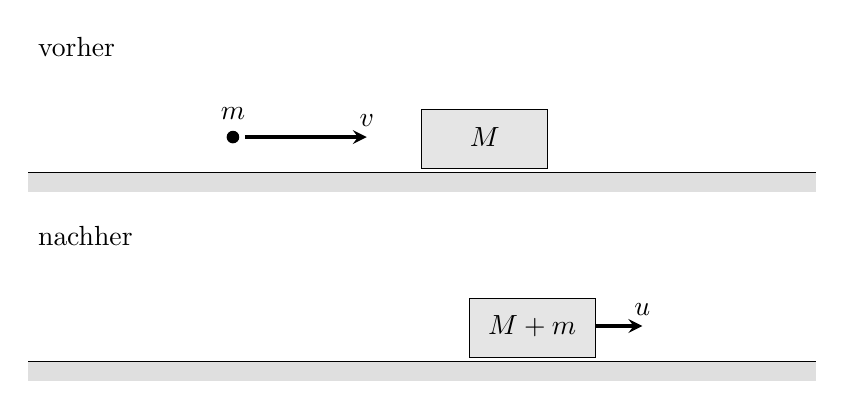
\begin{tikzpicture}[>=stealth]
 \fill[gray!25] (0,-0.25) rectangle (10,0);
 \draw (0,0) -- (10,0);
 \node[anchor=west] at (0,1.6) {vorher};
 \draw[fill=gray!20] (5,0.05) -- (6.6,0.05) -- (6.6,0.8) -- (5,0.8) -- cycle;
 \node at (5.8,0.45) {$M$};
 \fill (2.6,0.45) circle (0.08);
 \node[above] at (2.6,0.55) {$m$};
 \draw[->, very thick] (2.75,0.45) -- (4.3,0.45) node[above] {$v$};
 \fill[gray!25] (0,-2.65) rectangle (10,-2.4);
 \draw (0,-2.4) -- (10,-2.4);
 \node[anchor=west] at (0,-0.8) {nachher};
 \draw[fill=gray!20] (5.6,-2.35) -- (7.2,-2.35) -- (7.2,-1.6) -- (5.6,-1.6) -- cycle;
 \node at (6.4,-1.95) {$M+m$};
 \draw[->, very thick] (7.2,-1.95) -- (7.8,-1.95) node[above] {$u$};
\end{tikzpicture}
\end{center}

Die Kugel bleibt stecken, Kugel und Gleiter bewegen sich danach gemeinsam (vollständig unelastischer Stoss). Impulserhaltung:
\begin{align}
 m\,v &= \left(m+M\right)u
\end{align}
Also war die Kugel
\begin{align}
 v &= \vKgF \\
   &= \frac{\mKg+\mGl}{\mKg}\cdot\uGl \\
   &= \vKg \approx \result{\vKgP{0}{2}}
\end{align}
schnell.
